

\documentclass[tikz,border=10pt]{standalone}
\usepackage{amsmath}
\usetikzlibrary{automata,positioning}
\usetikzlibrary{arrows.meta}

\begin{document}
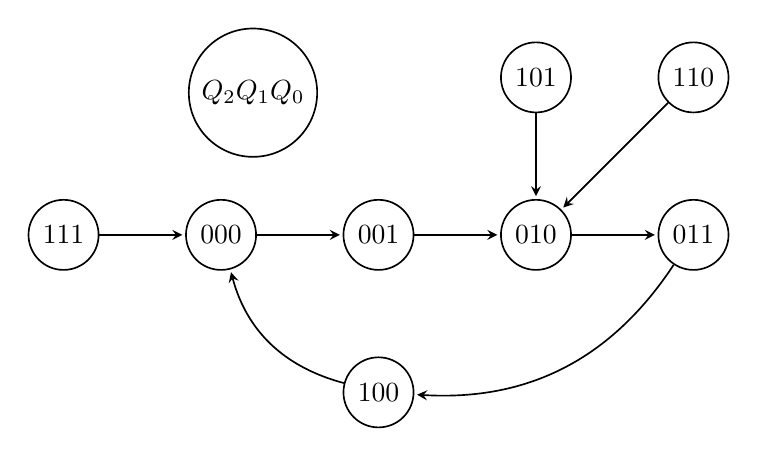
\begin{tikzpicture}[->,>=stealth,shorten >=1pt,auto,node distance=2cm,
                    semithick]

  \node[state] (S0)                     {$000$};
  \node[state] (S1) [right of = S0]     {$001$};
  \node[state] (S2) [right of = S1]     {$010$};
  \node[state] (S3) [right of = S2]     {$011$};
  \node[state] (S4) [below of = S1]     {$100$};
  \node[state] (S5) [above of = S2]     {$101$};
  \node[state] (S6) [right of = S5]     {$110$};
  \node[state] (S7) [left of = S0]      {$111$};

  \node[state] (dp) [above right = 0.9cm and -0.5cm of S0] {$Q_2 Q_1 Q_0$};

  \path
        (S0) edge              node {} (S1)
        (S1) edge              node {} (S2)
        (S2) edge              node {} (S3)
        (S3) edge [bend left]  node {} (S4)
        (S4) edge [bend left]  node {} (S0)
        (S5) edge              node {} (S2)
        (S6) edge              node {} (S2)
        (S7) edge              node {} (S0)
  ;
\end{tikzpicture}

\end{document}
